%
% Installation
%

%%%%%%%%%%%%%%%%%%%%%%%%%%%%%%%%%%%%%%%%%%%%%%%%%%%%%%%%%%%%%%%%%%%%%%%%%%%%%%%
%                  <--- 80 characters width --> 		                      %
%%%%%%%%%%%%%%%%%%%%%%%%%%%%%%%%%%%%%%%%%%%%%%%%%%%%%%%%%%%%%%%%%%%%%%%%%%%%%%%

\chapter{Installation}
\label{chap:vlet_installation}

\section{Installation requirements}

The VL-e Toolkit has the minimal following installation requirements:
\begin{itemize}  
   \item SUN Java 1.6 JRE (Java Runtime Environment) or JDK is recommended.   
   \item Either Windows 2000/XP/7 or a recent Linux distribution (2.6 kernel)
   \item Other Java 1.6 capable platforms might work as well, but not all
   architectures have been tested. (Mac Os has been reported to work as well).\\
   Alternative Java implementations like 'gcj'  and 'openjdk' might not fully
   support Swing applications which is mandatory for the VBrowser. 
 \end{itemize} 

Also, to be able to access grid resources, you MUST have a grid certificate. 
For instructions how to get one, see:
\url{http://certificate.nikhef.nl/request} or ask your local grid administrator. 

\section{Unpacking}

 Unzip the package with winzip (windows) or gunzip (linux). 
 The installation directory into which you installed it, will be referred to
 as \VLETINSTALL. \\
 \\
 Default installation path on Linux (system wide) installation could be: \\
 \\
 \tab \path{/opt/vlet}\\
 \\
 The installation path on Linux for non system administrators, could be:\\ 
 \\
 \tab \path{\$HOME/vlet}\\
 \\%%$
 Default installation path for a windows (system wide) installation
 could be: \\
 \\
 \tab \path{C:\vlet}\\ 
 \\	
 As users do not need write access to the installation path nor administrator
 rights to install or run parts of the VL-e Toolkit, any user can install it 
 at the desired place he or she wants to.\\
 After unpacking the VL-e toolkit can be used directly by starting the desired
 application or tool from the \path{VLET_INSTALL/bin} directory. Most users don't have 
 to configure their installation and should be able to use the tools right out
 of the box.
 For custom configurations, see the next chapters for an explanation of
 optional properties and installation settings.\\
 
 \subsection{Quick Installation Steps}
 Quick install steps for the impatient are as follows:
 
 \begin{itemize} 
   \item Unzip the vlet distribution. 
   \item Put your personal grid certificate (userkey.pem and usercert.pem) in
         your \HOME/.globus directory. Create the \path{.globus} directory if
         it doesn't exists yet. 
   \item Optionally create a shortcut to \path{VLET_INSTALL/bin/vbrowser.exe}
         (for \windows) and copy the shortcut to your desktop.
   \item Start \path{vbrowser.sh} or \path{browser.exe} from
          \path{VLET_INSTALL/bin} (or use shortcut). 
   \item Optionally, the \path{vbrowser.jar} can be used to directly start the
          vbrowser using any Java Environment (for Mac OS this is the only
          supported way) as follows: \path{java} \path{-jar} \path{vbrowser.jar}
   \item Configure firewall settings by right-clicking (alt mouse button) on the 
         \myvle\ icon seen in Figure \ref{fig:myvle_icon}, select \Menu{properties} and set \Menu{passiveMode} to
   \Menu{true} for firewalled users, or specify an incoming port range if you
         allow incoming tcp/ip connections.
	  
	  \begin{figure}[htbp]
	    \centerline{
\includegraphics[scale=1.0]{vle-world}}
	    \caption{The \myvle\ Icon}
	    \label{fig:myvle_icon}
	  \end{figure}

   \item Optionally put extra CA certificates in your  
         \path{HOME/.vletrc/certificates} directory if CA certificates can't be
         found. This is necessary for non-\dutchgrid\ sites. 
 \end{itemize} 
 
\subsection{Directory structure}

Below an overview of the directory structure of the installation. Only relevant
files and directories are listed here. 

\begin{boxedlisting}
\begin{verbatim}
# Directory structure of VLET distribution: 

ReleaseNotes.txt        # latest release notes.
README.txt              # general README.
INSTALL.txt             # extra installation notes. 
ReleaseNotes.txt        # latest release notes.
LICENCE.txt             # Apache Licence 2.0.
bin/                    # scripts and (binary) executables.
bin/vbrowser.sh         # UNIX (Linux) VBrowser startup script. 
bin/vbrowser.exe        # Windows VBrowser startup executable.
bin/vbrowser.jar        # Java executable jar file.
etc/                    # configuration files. 
etc/vletrc.prop         # installation settings.  
etc/vletenv.sh          # extra Unix/Linux environment settings. 
etc/certificates/       # root CA certificates needed for authentication of 
                          remote hosts.
doc/                    # documentation and Java API (javadoc) files. 
lib/                    # libraries and needed jar files including icons.
lib/plugins             # custom viewers and plugins both for VDrivers and 
                          Viewer Plugins.  
lib/icons               # custom icons. 
lib/icons/mimetypes     # custom mimetype icons.
py/                     # Java Python (Jython) examples.  
\end{verbatim}
\end{boxedlisting}
 
\subsection{Configuring the installation}

 The next sections explains how to configure the default settings in your
 installation. 
 Most settings can be changed interactively through the \vbrowser\ as well.
 You can do this by right-clicking (or use alt-mouse button) on
 the \myvle\ icon or specified resource.
\par
 See the file \VLETCONF\ for (advanced) installation configuration. All the
 variables can also be specified for each user in the
 \path{HOME/.vletrc/vletrc.prop} which overrides default installation settings. (see
 Section: \ref{sec:user_configuration}). As this file changes per distribution,
 see the comments before each property and which are the optimal defaults for your
 distribution and your environment. \\


\section{Configuring Grid Certificates}

\subsection{Configuring your personal grid certificate}
\label{sec:user_configuration}

The next paragraphs explain where you can find/store your grid certificate
depending on the operating system you are using. 

\subsubsection{Grid certificate directory for \Linux}

 The default location to store your grid certificate for \Linux\ is:
 
 	\tab \path{HOME/.globus}  

 This is the location where the Globus Commodity Grid Toolkit (CoG) stores its
 configuration files. This location is the recommended place for Linux and
 windows users to store their grid certificates (See next section how to find
 your windows home).
 
\subsubsection{Grid certificate directory for \windows}
 
 The default location for \windows\ (XP) could be (depending on the default
 user's home): 
 
	 \tab \Path{C:\bsl WINDOWS\bsl profiles\bsl (Your User Name)\bsl .globus}

 The \Path{C:\bsl WINDOWS} part is the prefix where windows is installed. 
 The \Path{.globus} is the directory where the Globus Commodity Grid
 Toolkit (CoG) stores its  configuration files. \\
 If you don't know how to find your Windows \HOME\ you can also just start the
 \vbrowser\ and your home path will be the first resource under the \LocalSys\ icon. 
 This home resource is recognizable by the folder icon
 which has a little house in it as you can see in Figure \ref{fig:home_folder_in_tree}.
 
  \begin{figure}[htbp]
  \centerline{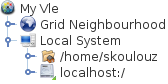
\includegraphics[scale=1.0]{home_folder_tree}}
  \caption{Your HOME folder under window and Linux}
  \label{fig:home_folder_in_tree}
 \end{figure}
 
 Alternatively you could store your certificates into
 another location, or keep a copy, for example the following location:
 
 	 \tab \Path{C:\bsl My Documents\bsl globus}
 
 When installing your grid certificates into another location than the default, 
 you need to configure the VBrowserto search for this location. 
 This will be explained in Section \ref{sec:grid_proxy_configuration}. 
 
\subsubsection{Your Grid Certificate files}

 The files which must be present in your globus certificate directory
 (\path{HOME/.globus}) are:

 \begin{itemize} 
   \item \File{userkey.pem} : 
     Your \Emph{private} grid certificate. Never share this file with anyone. If you 
     loose this file, you'll need to reapply for a new grid certificate. 
   \item \File{usercert.pem} : 
     Your \Emph{public} grid certificate. This file is send over the internet to 
     identify you as the person defined in your grid certificate. Together
     with the \File{userkey.pem} it forms your \Emph{public-private} keypair. 
  \end{itemize} 
  
 For more about \Emph{public-private} keypair encryption, see: \cite{PKCS}.
 
 Optionally this directory may contain the following files: 

 \begin{itemize} 
   \item \File{cog.properties} : 
     This file contains the Globus Commodity Grid (CoG) Toolkit properties.
 \end{itemize} 
 
 \Note{Note}: The \File{cog.properties} file is \Emph{always} stored in the default
 globus configuration directory (\Path{.globus}) in your \HOME\ directory. If this 
 file is present it will override any configurations made in \VLETCONF\ or 
 \path{HOME/.vletrc/vletrc.prop}

\subsection{Configuring host certificates} 

The default place to store host certificates under \Linux\ is:\\

	\tab \Path{/etc/grid-security/certifates}\\
	
If you don't have the rights to add/install certificates to this place, you can 
add new certificates to the following location: 

	\tab \VLETINSTALL\path{/etc/certificates}

Or to add CA certificates to your user environment put them in: 

	\tab \path{HOME/.vletrc/certificates} 

Certificates added to the above locations are loaded automatically
when starting tools from the VL-e toolkit. 
For windows users replace the \path{HOME} variable with your user profile
location. 

For access to \dutchgrid\ sites, no extra configuration should be necessary. To
access other (non \dutchgrid) sites, add your root CA certificate to one of
the above custom locations. 

More information about Grid Certificates can be found here: \cite{288111}


\subsection{Advanced certificate configuration settings}
See the installation file \path{VLET_INSTALL/etc/vletrc.prop} or the user
configuration file \path{HOME/.vletrc/vletrc.prop} for advanced
grid configuration settings. 
Explanation of these properties can be found in Section:\ref{sec:properties})

%%%
%%% Section 
%%%

\section{Properties and configuration settings}
\label{sec:properties}

In the next (sub)sections an overview of the most important settings which can
be specified either installation wide in the \VLETCONF\ file or in the user's
configuration file \VLETUSERCONF. 


%%% --------Obsolete-------------------
% \subsection{Configuring default Resource settings} 
% 
%  The installation file \path{VLET_INSTALL/etc/vletrc.prop} also contains default
%  resource settings for SRB and LFC. When creating a new Resource Location, the default 
%  settings from this file will be used. This file contains \Emph{installation} wide 
%  settings and  may not contain user specific configuration details.\\
%  The location of this file is: 
% 
% 	\tab \path{VLET_INSTALL/etc/vletrc.prop}
% 	
% For example, the default SRB configuration to access the SRB server at SARA is: 
% 
% \begin{boxedlisting}
% \begin{verbatim}
% ##
% # File    : vletrc.prop 
% # Location: $VLET_INSTALL/etc/vletrc.prop 
% # ---
% 
% # ...  
% 
% # Default SRB settings file for SRB server at SARA 
% 
% # Default SRB host at SARA :
% srb.hostname=srb.grid.sara.nl
% srb.path=/VLENL/home
% srb.port=50000
% srb.mdasCollectionHome=/VLENL/home
% srb.mdasDomainHome=vlenl
% srb.mdasDomainName=vlenl
% srb.defaultResource=vleGridStore
% #srb.username=
% srb.mcatZone=VLENL
% # set to true when behind a firewall (Default)
% # if incoming connection are allowed set to 'false'
% srb.passiveMode=true
% #this string MUST match the Enum Value for 'GSI_AUTH'
% srb.AUTH_SCHEME=GSI_AUTH
% 
% # end srbsettings.prop file 
% \end{verbatim}
% \end{boxedlisting}  
%  
% \Note{Note}: Do NOT put a username in this file, since this file contains
% installation wide settings. \\
% 
% Before users will be able to access an SRB server, they have to create/modify
% an SRB server location interactively by using the VBrowser (see Chapter: \ref{chap:vbrowser}).
% The above mentioned file is \Emph{only} for default installation settings.
% To customize your personal environment you can copy the above settings in your
% own \path{HOME/.vletrc/vletrc.prop} file. In that case you can fill in your
% (default) SRB user name in the configuration file. 

\subsection{Firewall settings}
\begin{itemize}  
   \item \Variable{firewall.portrange}: Allowed incoming port range for
   hosts which have a 'hole' in their firewall. For example:\\
    
   \tab \Variable{firewall.portrange=20000,25000}\\
   
   Leave empty if no range is defined.\\
     
   \item \Variable{passiveMode}: Set to true when incoming connections are NOT
   allowed (firewall port-range will be ignored!). For example:\\

   \tab \Variable{passiveMode=true}\\
  
\end{itemize} 
\Note{Note:} if you set \Variable{passiveMode} to \Variable{true}, \Emph{all} server 
configurations will use passiveMode. Keep this setting to \Variable{false} if
you want to specify this option per server. This is the case when you have
file servers which are behind the same (company) firewall and are not blocked
when accessing them from your desktop.\\

\Note{Performance note:} Allowing incoming connections can considerably speed up
file transfer and is recommended for large file transfers even for low bandwidth
connections and especially for connections which have a high (tcp/ip) latency. 

\subsection{Grid proxy and grid certificate locations}
\label{sec:grid_proxy_configuration}

You can specify alternate locations to your Grid Certificate and Proxy Location.
Beware that when you specify these setting in the installation configuration
(\Path{VLET\_INSTALL/etc/vletrc.prop}), you'll be specifying this for \Emph{all} users.\\
Use \Path{HOME/.vletrc/vletrc.prop} for personalized settings. You can copy
any installation property from the installation file in to your own user
property file to customize your environment. \\
\\
\begin{itemize}  
   \item \Variable{grid.proxy.location}: absolute path to grid proxy location or
   relative from user's \HOME. For example (absolute path):\\
   
   \tab \Variable{grid.proxy.location=/etc/ptdeboer\_proxy.x509}\\
   
   or a location relative to the user's \HOME:\\
    
   \tab \Variable{grid.proxy.location=mycerts/myproxy.x509}\\

   or (preferably) leave empty to use (CoG/globus) defaults. 
   
   \item \Variable{grid.certificate.location}: Relative path (to user's home)
   or absolute path to the directory containing your grid certificates (both
   public and private keys). Leave empty to use (globus) defaults. \\
    
   \tab \Variable{grid.certificate.location=.globus}\\
   
   Above setting is the default location as used by CoG/globus. 
  
\end{itemize} 


\subsection{Command line options and environment variables}

All properties can be set by specifying them as extra arguments on the command
by using the -D command as follows: \Variable{-D\lt variable \gt=\lt value \gt }.
The order in which properties are checked is as follows (higher priority first):

\begin {itemize}
  \item Command line options \Variable{-D\lt variable \gt=\lt value \gt}
  \item Environment variables. 
  \item User configuration file: \VLETUSERCONF 
  \item Installation configuration file: \VLETCONF 
  \item Hard-coded defaults (for configuration-less environments)
\end{itemize}
